\documentclass[11pt,a4paper]{article}
\usepackage[T1]{fontenc}
\usepackage[utf8]{inputenc}
\usepackage{lmodern}
\usepackage{microtype}
\usepackage[margin=2.5cm]{geometry}
\usepackage{setspace}
\usepackage{booktabs}
\usepackage{array}
\usepackage{tabularx}
\usepackage{amsmath}
\usepackage{graphicx}
\usepackage[natbibapa]{apacite}
\usepackage[hidelinks]{hyperref}
\usepackage{xcolor}
\newcommand{\todo}[1]{\textcolor{red!70!black}{[#1]}}
\newcommand{\code}[1]{\texttt{#1}}
\newcolumntype{L}[1]{>{\raggedright\arraybackslash}p{#1}}
\newcolumntype{Y}{>{\raggedright\arraybackslash}X}

\title{Generalising D\"orner's selection threshold to a limited-capacity workspace: an incumbency bonus makes contents history-dependent in a PSI island agent}
\author{Alec Sproten\\[0.5ex]
\small Baden-Wuerttemberg Cooperative State University (DHBW) Ravensburg, Germany\\
\small ORCID: \href{https://orcid.org/0000-0001-8660-2173}{0000-0001-8660-2173}\\[0.5ex]
\small Corresponding author: Alec Sproten, \href{mailto:alec.sproten@aol.be}{alec.sproten@aol.be}}
\date{Preprint, submitted to \emph{Adaptive Behavior}\\[0.5ex]\small Words: about 5{,}900 (main text with captions and declarations, without references); figures: 3; tables: 5}
\begin{document}
\maketitle

\begin{abstract}
In D\"orner's PSI theory a new motive replaces the current one only if it is stronger by more than a selection threshold that grows with arousal. The aim of our study was to test whether the same additive margin stabilises every content that competes for a limited-capacity workspace. In a reconstruction of D\"orner's island agent we compared five conditions over 100 paired lives each, following an analysis plan committed in advance: no workspace, a bonus equal to the threshold for all contents, for motives only, a constant bonus of the same mean size, and no bonus. Relative to the workspace without bonus, the general bonus reduced switches of the leading goal from 8.5 to 3.7 per 100 cycles, and relative to a bonus for motives only it raised the dwell time of other contents from 13.2 to 33.7 cycles. Without workspace, the agent switched its leading goal less often than it did in any workspace condition. In a diagnostic rerun, most cycles in which the bonus changed the selection had tied candidates, and a strictly weaker incumbent was kept in about 6\,\% of cycles; a bonus of 0.02 produced most of the effect, and with random instead of alphabetical tie-breaking the workspace without bonus switched its leading goal 68 times per 100 cycles. A constant bonus behaved like the arousal-coupled one, and no measure of plan failure, opportunistic satisfaction or survival differed reliably between conditions. In this world, the bonus makes the workspace history-dependent and prevents oscillation among equivalent options.
\end{abstract}

\noindent\textbf{Keywords:} PSI theory, global workspace, selection threshold, hysteresis, action selection, stability-flexibility dilemma


\section{Introduction}

An agent that pursues goals in a changing environment has to shield its current intention against distraction and still remain open to opportunities and dangers. Action control theory describes the shielding of intentions \citep{kuhl1985volitional}, the Rubicon model the volitional mindset that follows a decision \citep{heckhausen1987thought}, and research on cognitive control a stability-flexibility dilemma whose balance is shifted by affect and reward \citep{goschke2014emotional,dreisbach2004positive,hommel2015between}. Computational accounts treat the dilemma as one reason why the capacity for control is limited \citep{musslick2021rationalizing} and model it as the gating of working memory between maintenance and updating \citep{oreilly2006making}.

D\"orner's PSI theory gives the dilemma a computable form for motives \citep{doerner2002mechanik,doerner2013psi}. A motive takes over only if it exceeds the current motive's strength by more than a selection threshold, which is the product of arousal and a constant. The current motive thereby ``defends'' itself, and an aroused agent becomes more persistent \citep[pp.~97--98]{doerner2002mechanik}. D\"orner also links the threshold to attention: a high threshold keeps the number of background goals small, and background goals constitute the breadth of attention \citep[p.~99]{doerner2002mechanik}. Simulations reported in the same book varied the threshold between 0.1 and 0.8 and found that a higher threshold led to more nucleotides collected and more locations visited, but also to more breakdowns \citep[pp.~241--248]{doerner2002mechanik}. Bach's reconstruction of PSI describes the threshold as a bias added to the currently selected motive and, in the MicroPsi agent, as a bonus for the selected intention ``which adds a hysteresis that keeps the active intention more stable''; the MicroPsi architecture also contains an access memory labelled as workspace \citep[sections 4.6.2, 6.2.3 and figure 8.2]{bach2009principles}.\footnote{Quotation, section and figure numbers follow the pre-publication manuscript of January 2008 that was available to us; the corresponding passages of the printed edition have not been compared.} OpenPsi passes attentional value, scaled by the selection threshold, to the goal atoms that were most valued in the previous cycle \citep{cai2011openpsi}. The idea that the selection threshold is a form of hysteresis, and that it can act on attention, is therefore not new.

Global workspace theory locates the competition between contents in a limited-capacity workspace whose winners are made available to many specialised processes \citep{baars1988cognitive,dehaene1998neuronal,mashour2020conscious}. In neuronal workspace models, the winning coalition sustains itself through recurrent activity once it has ignited, which gives it stability \citep{dehaene1998neuronal,mashour2020conscious}; LIDA and Shanahan's architecture implement persistence through the dynamics of competing processes \citep{franklin2014lida,shanahan2006cognitive}. Recent artificial agents use a learned bottleneck \citep{goyal2022coordination,vanrullen2021deep}; in the agent of \citet{dossa2024design}, the previous workspace state enters both the attention mechanism, as a query, and the recurrent update, as the hidden state of a gated recurrent unit, so that persistence is learned rather than imposed. Table~\ref{tab:prior} summarises these mechanisms as far as the cited descriptions state them.

\begin{table}[t]
\centering
\caption{How prior architectures carry the content of a workspace or an intention from one step to the next, as described in the cited sources.}
\label{tab:prior}
\small
\begin{tabularx}{\textwidth}{L{0.26\textwidth} Y}
\toprule
Architecture & Persistence of the current content \\
\midrule
PSI \citep{doerner2002mechanik} & Selection threshold (arousal $\times$ constant) protects the current motive \\ \addlinespace
MicroPsi \citep{bach2009principles} & Bonus equal to a selection threshold for the active intention, described as hysteresis; access memory as workspace \\ \addlinespace
OpenPsi \citep{cai2011openpsi} & Attentional value scaled by the threshold passed to the goals most valued in the previous cycle \\ \addlinespace
Neuronal workspace \citep{dehaene1998neuronal} & Self-sustaining recurrent activity of the ignited coalition \\ \addlinespace
LIDA, Shanahan \citep{franklin2014lida,shanahan2006cognitive} & Dynamics of competing coalitions or processes \\ \addlinespace
Learned bottlenecks \citep{goyal2022coordination,dossa2024design} & Learned attention and recurrent state; previous workspace as query and hidden state in \citet{dossa2024design} \\ \addlinespace
This study & One explicit additive bonus for every incumbent content, of any kind, in a capacity-limited selection; varied experimentally \\ \addlinespace
\bottomrule
\end{tabularx}
\end{table}

What we add is narrower than a new principle. The aim of our study was to find out whether D\"orner's rule, generalised in this way, stabilises the contents of a workspace and what it changes in the agent's behaviour. We apply one explicit additive rule, D\"orner's threshold, to all kinds of content in a capacity-limited selection, vary it experimentally against controls that remove it, restrict it to motives, decouple it from arousal or keep the workspace away entirely, and test the consequences in the program in which the threshold was conceived. The hypothesis, fixed before the runs, was that such a general bonus would (1) make all workspace contents more stable, (2) make their stability depend on arousal, and (3) make the workspace history-dependent. We use a reconstruction of D\"orner's island program in Python \citep{paper1} in its modern mode, in which implementation properties of the original that are not part of its description are switched off.

\section{Model}

\paragraph{The agent.} In each behaviour cycle the PSI agent updates its needs, selects the current motive with the selection threshold, builds a goal list from the goals of the current need and from background goals of other needs, and then tries in turn to find a goal in the current situation (\code{LookAround}), to run an automatism, to make and execute a plan, or to explore by trial and error (\code{WhatCouldBeDone}) \citep{doerner2002mechanik}. Arousal, the resolution level and the selection threshold modulate these processes; in the island configuration the threshold equals $0.1$ times arousal. On this island the current motive is almost always the need for nucleotides \citep{paper1}.

\paragraph{The workspace.} Once per cycle, after the goal list has been built, candidates compete for the workspace. Table~\ref{tab:kinds} defines each kind of content: which neuron represents it, how its strength is computed, how long it remains a candidate, and which parts of the regulation read it. A neuron enters the competition once, with its strongest reading; on equal strength it counts as the most specific kind (plan before memory before goal). The capacity is $K = \mathrm{round}(2 + 5 r)$, where $r$ is the resolution level; in the runs reported here $K$ took the values 4, 5 and 6 (in condition B in 26\,\%, 71\,\% and 2\,\% of cycles). The need of the current motive always holds one place; it is chosen by the motive selection of PSI and does not compete in the workspace selection. The remaining $K-1$ places go to the candidates with the largest strength plus bonus, where the bonus applies only to contents that were in the workspace in the previous cycle; equal sums are ordered by the name of the neuron.

\begin{table}[t]
\centering
\caption{Kinds of workspace content. ``Next cycle'' means that the content is read by the regulation of the following cycle; ``same cycle'' means that it is read after the selection in the cycle in which it was selected.}
\label{tab:kinds}
\footnotesize
\begin{tabularx}{\textwidth}{L{0.12\textwidth} L{0.17\textwidth} L{0.27\textwidth} L{0.15\textwidth} Y}
\toprule
Kind & Neuron & Strength & Candidate while & Read by \\
\midrule
Current motive & Need of the current motive & Motive strength & Always (reserved place) & Not read; motive selection is unchanged \\ \addlinespace
Other motives & Need neurons & Motive strength of the cycle & Need active & Not read \\ \addlinespace
Goal & Goal schema & Need activity $\times$ need weight $\times$ goal-link weight; intermediate goals inherit the value of their end goal & Linked to a need or in the goal list & Goal list, front (next cycle) \\ \addlinespace
Object & Object of the current situation & Larger of novelty $1/(1+n)$ and threat via aversion links & In the current situation & \code{LookAround} first if also a goal; \code{WhatCouldBeDone} always (same cycle) \\ \addlinespace
Memory & Situation recalled by \code{Association} & Value of the goal it contains & Until the next successful recall & Goal list (next cycle) \\ \addlinespace
Plan & End of the last executed plan & Value of the goal planning found there & Until the next plan & Goal list (next cycle) \\ \addlinespace
\bottomrule
\end{tabularx}
\end{table}

One cycle thus runs as follows. (1) Motivation selects the current motive. (2) \code{GoalGen} builds the goal list. (3) Goals, memories and plan ends that were selected in the previous cycle are placed at the front of the goal list; those that \code{GoalGen} did not add are added with link weight 1. (4) The workspace selection runs and is logged. (5) The regulation runs; \code{LookAround} and \code{WhatCouldBeDone} read the objects selected in step 4. Candidate strengths are read without side effects. With the workspace switched off, the protocols of 20 lives were byte-identical to those of the modern mode without workspace.

\paragraph{Hysteresis of the selector.} Consider one free place, a candidate with strength $x$, a rival with strength 0 and a bonus $b > 0$. If the rival holds the place, the candidate enters only when $x > b$; if the candidate holds it, it stays as long as $x > -b$. For $-b < x < b$ the outcome depends on which candidate held the place before. The selection operator therefore has a hysteresis band of width $2b$, and whether this band matters depends on how often the strengths of competing candidates differ by less than $b$. Whether the closed loop of agent and world shows hysteresis in a stronger sense, with several stable states for the same external situation, is a different question that this study does not address.

\paragraph{Relation to global workspace theory.} Of the indicator properties that \citet{butlin2023consciousness} derive from the theory, our extension implements a limited-capacity selection with an attention-like competition (GWT-2) and passes its contents to three procedures of the regulation (a partial form of GWT-3, since perception, memory search and planning still operate on information outside the workspace). Its capacity depends on the agent's state, but it does not query modules in succession as GWT-4 requires. We therefore study an extension oriented towards global workspace theory and make no claim to a complete workspace architecture.

\paragraph{Conditions.} The five conditions differ only in the bonus. In A there is no workspace. In B every incumbent receives a bonus equal to the current selection threshold. In C only motives receive it. In D every incumbent receives a constant bonus of 0.064642, the mean threshold over all 18{,}095 cycles of 20 lives of A. In E there is no bonus. In D and E, motive selection also uses the constant and no bonus respectively; the release of a motive, which requires arousal above the threshold, is the same in all conditions. In B the realised bonus had a mean of 0.0656 and a standard deviation of 0.0100 (range 0.034 to 0.100).

\section{Design and analysis}

Each condition was run for seeds 1001 to 1100, one life per seed to a model age of 5{,}000{,}000, which took between 369 and 2{,}618 cycles. Conditions were paired by seed, and the unit of analysis is the seed. From the per-cycle logs we computed the observed dwell time of contents (W1, the mean length of uninterrupted stays per life, in cycles), switches of the leading goal, the first entry of the goal list after step 3, per 100 cycles (W2b), failed plan executions per 100 cycles (W3, plans whose execution ended without reaching the goal, for whatever reason), satisfactions of needs other than the current motive per 100 cycles (W4), the rank correlation between arousal at entry and dwell time for contents other than motives (W5), and the share of cycles in which the selected set differs from the selection without bonus (W6, a manipulation check). Stays still running at the end of life count with their length so far, and a stay is assigned to the kind of its content at entry.

The confirmatory hypotheses were that B, compared with E, has fewer leading-goal switches (H1), fewer failed plans (H2), fewer opportunistic satisfactions (H5) and more history dependence (H6); that W5 is larger in B than in D (H3); and that non-motive dwell time is longer in B than in C (H4). The plan stated that the core claim would count as supported if H1, H3 and H4 were significant in the predicted direction. For each hypothesis we estimated the mean of the per-seed differences with a percentile bootstrap interval (10{,}000 resamples) and tested it with a two-sided sign-flip permutation test (10{,}000 permutations; this test assumes that the paired differences are symmetric about zero under the null hypothesis), both with fixed seeds, and corrected the six $p$ values with Holm's procedure at $\alpha = .05$. The intervals are pointwise. All six tests had 100 valid pairs. Survival and performance measures (P1 to P6) were compared between each workspace condition and A as secondary, descriptive analyses with Holm's correction within each condition.

\paragraph{Chronology.} Table~\ref{tab:chronology} lists the commits of the analysis plan and of the code. A functional test of 300 cycles in all conditions preceded amendment 1, which moved H1 from switches of the current motive to switches of the leading goal, because data of condition A available before the plan showed that the motive almost never changes. A first screening run was stopped after three completed lives of B, when the logs showed that memories and plans never entered the workspace; amendment 3 corrected their valuation and changed W1 to count stays per neuron, assigned to the kind at entry, and the three lives were discarded. The screening on seeds 1001 to 1020 was not limited to a check for errors. Its evaluation, committed before the confirmatory runs began, contained the hypothesis tests and effect sizes for these seeds and a written assessment: large effects for H1, H4 and H6, no difference for H3, H2 and H5, and the expectation that the core claim would not be supported if H3 remained null. After this evaluation, neither the hypotheses, the measures, the decision rule, the analysis code nor the code of the agent was changed (no commit touched the plan, \code{src/} or the analysis script between \code{0d78571} and the confirmatory analysis). As the plan prescribed, the 20 screening lives are part of the confirmatory sample of 100; the confirmatory analysis is therefore the planned analysis of 100 seeds of which 20 had already been analysed, not an independent replication. The analysis of the 80 seeds 1021 to 1100 alone, reported below, was computed after the confirmatory analysis.

\begin{table}[t]
\centering
\caption{Chronology of the study (commit times UTC, 11 November 2026). The code of the confirmatory runs is commit \code{c0194b6}.}
\label{tab:chronology}
\footnotesize
\begin{tabularx}{\textwidth}{l l Y}
\toprule
Time & Commit & Change, and data seen up to then \\
\midrule
09:12 & \code{68bd418} & Analysis plan, before any run with workspace; data of A (modern mode without workspace) existed \\ \addlinespace
09:18 & \code{79e228b} & Workspace code; functional test of 300 cycles of seed 1001 in all conditions follows \\ \addlinespace
09:31 & \code{b82aca9} & Amendment 1: H1 on leading-goal switches (motive switches zero in A and in the functional test) \\ \addlinespace
10:00 & \code{4cb532d} & A rerun with workspace log (1001 to 1020), identical to the baseline; amendment 2 fixes the bonus of D \\ \addlinespace
10:12 & \code{c0194b6} & Amendment 3: valuation of memories and plan ends, W1 per neuron; three screening lives of B discarded \\ \addlinespace
12:04 & \code{0d78571} & Screening 1001 to 1020 completed; hypothesis tests, effect sizes and a written assessment of the 20 seeds committed; confirmatory runs started without changes to plan, analysis code or agent \\ \addlinespace
19:56 & \code{523588f} & Confirmatory analysis of 1001 to 1100 \\ \addlinespace
\bottomrule
\end{tabularx}
\end{table}

\section{Results}

All 400 lives of conditions B to E completed. Table~\ref{tab:hyp} shows the confirmatory tests. H1, H4 and H6 were significant in the predicted direction; H2, H3 and H5 were not. By the criterion fixed in advance, the core claim is not supported.

\begin{table}[t]
\centering
\caption{Confirmatory tests over seeds 1001 to 1100 ($n = 100$ pairs each). Difference: mean of per-seed differences, condition B minus the comparison condition, with pointwise 95\,\% bootstrap interval; $p$ values Holm-adjusted across the six tests. Units: W1 cycles; W2b, W3, W4 events per 100 cycles; W5 Spearman correlation; W6 share of cycles.}
\label{tab:hyp}
\footnotesize
\begin{tabularx}{\textwidth}{l Y l r r l r}
\toprule
 & Measure & Contrast & Mean B & Difference & 95\,\% CI & $p_{\mathrm{Holm}}$ \\
\midrule
H1 & W2b leading-goal switches & B $-$ E & 3.74 & $-4.78$ & $[-5.20, -4.34]$ & $<.001$ \\
H2 & W3 failed plans & B $-$ E & 2.97 & $-0.18$ & $[-0.44, 0.08]$ & .546 \\
H3 & W5 arousal at entry vs.\ dwell & B $-$ D & 0.156 & $0.011$ & $[-0.017, 0.040]$ & .791 \\
H4 & W1 dwell, non-motive & B $-$ C & 33.68 & $20.48$ & $[18.80, 22.23]$ & $<.001$ \\
H5 & W4 opportunistic satisfactions & B $-$ E & 11.88 & $-0.23$ & $[-0.72, 0.29]$ & .791 \\
H6 & W6 history-dependent cycles & B $-$ E & 0.371 & $0.371$ & $[0.357, 0.386]$ & $<.001$ \\
\bottomrule
\end{tabularx}
\end{table}

\paragraph{Stability relative to which baseline.} With the general bonus the leading goal changed 3.7 times per 100 cycles, without bonus 8.5 times. Non-motive contents stayed 33.7 cycles on average with the general bonus, 13.2 with a bonus for motives only and 13.0 without bonus, so a bonus for motives alone added nothing to the stability of other contents. The longer stays appeared for every kind at entry (Figure~\ref{fig:dwell}). The agent without workspace, however, changed its leading goal less often than it did in any workspace condition: in the 20 lives of A with a workspace log, 0.58 times per 100 cycles, against 3.67 in B and 8.08 in E for the same seeds (computed after the confirmatory analysis). Introducing the workspace with its broadcast thus made the head of the goal list more variable, and the bonus reduced this variability without bringing it back to the level of the agent without workspace. The stability we report is stability relative to a workspace without bonus.

\begin{figure}[t]
\centering
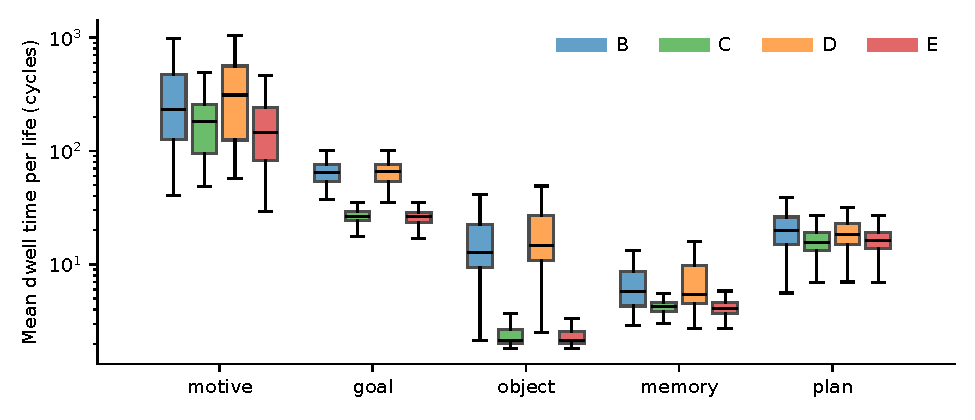
\includegraphics[width=\textwidth]{abbildungen/A2.pdf}
\caption{Mean observed dwell time per life by kind at entry and condition (100 lives per condition, each with all five kinds; boxes show quartiles, whiskers 1.5 interquartile ranges, outliers not shown, logarithmic scale). Number of stays per condition: B 11{,}399, C 27{,}000, D 11{,}071, E 27{,}211. Stays still running at the end of life count with their length so far. B: bonus equal to the selection threshold for all contents; C: for motives only; D: constant bonus for all; E: no bonus.}
\label{fig:dwell}
\end{figure}

\paragraph{History dependence.} In 37\,\% of the cycles of B the selected set differed from the selection without bonus, against 1\,\% in C and none in E, where the selection is by construction identical to the memoryless one. Figure~\ref{fig:timeline} illustrates the difference in one life fixed in advance as example. A one-step diagnostic shows where these departures come from. We reran B for seeds 1001 to 1020 with additional diagnostics in the log; the selected contents were identical to the confirmatory runs in all 20 lives. In 9.9\,\% of the 18{,}736 cycles, the last selected and the first rejected candidate had equal effective strength, and in 57\,\% their difference was smaller than the current bonus. The selection differed from the name-ordered memoryless selection in 36\,\% of cycles, but from every memoryless selection that resolves ties in any order in only 6.1\,\%. Most of the cycle-by-cycle departures from the name-ordered selection are therefore decisions among equally strong candidates, typically goals of the nucleotide need with identical values; in about one cycle in sixteen the bonus keeps a candidate that is strictly weaker than a rejected one. This decomposes the local difference measured by W6 within single cycles. It is not a causal decomposition of the longer stays or of behaviour, which arise in the feedback loop of agent and world.

\begin{figure}[t]
\centering
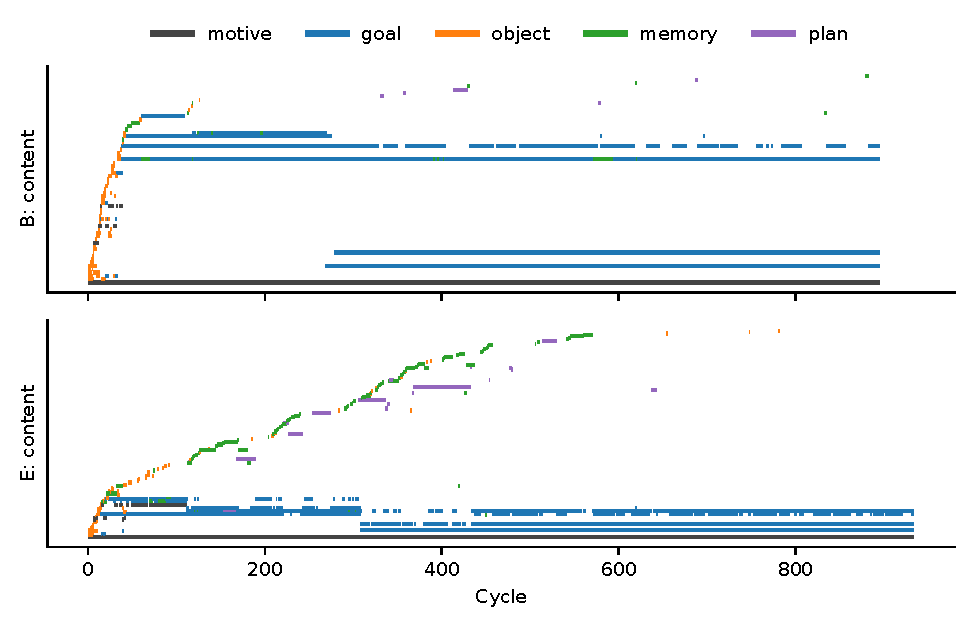
\includegraphics[width=\textwidth]{abbildungen/A4.pdf}
\caption{Contents of the workspace over one life (seed 1001, fixed in the analysis plan as example) in condition B (top) and E (bottom). Each row is one neuron, rows ordered by first entry within each panel; rows of the two panels do not correspond. Colour gives the kind of content in each cycle. Illustration of one life, not a test.}
\label{fig:timeline}
\end{figure}

\paragraph{Arousal.} Arousal at entry and dwell time correlated positively in B (mean $\rho = 0.156$ over lives) and similarly with the constant bonus (0.144); the difference was small and not significant. B and D were close on all workspace measures: leading-goal switches 3.74 and 3.75 per 100 cycles, non-motive dwell times 33.7 and 34.8 cycles, history-dependent cycles 37\,\% and 38\,\%. Figure~\ref{fig:arousal} shows the pooled distributions. The data are therefore compatible with no additional effect of coupling the bonus to arousal, but they do not show its absence: the coupled bonus varied little (standard deviation 0.010 around 0.066), the capacity, which also depends on arousal through the resolution level, took only three values, and arousal is itself a state of the agent that its behaviour changes. The positive correlation in both conditions cannot be attributed to a single path in this design.

\begin{figure}[t]
\centering
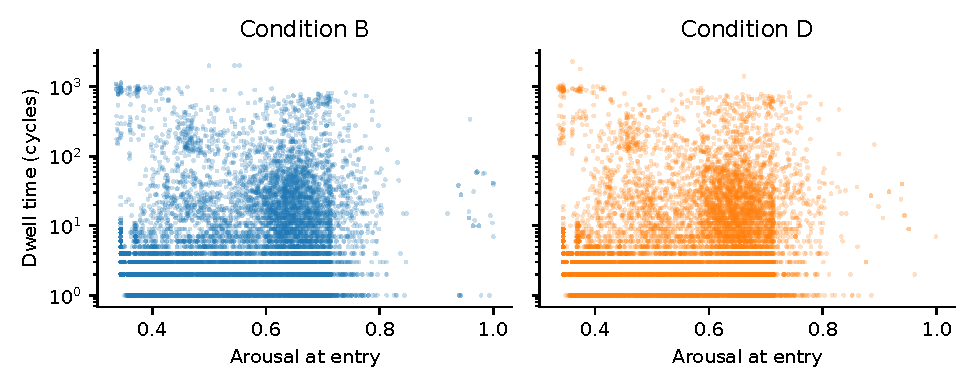
\includegraphics[width=\textwidth]{abbildungen/A3.pdf}
\caption{Arousal at entry and observed dwell time of all non-motive stays in B (10{,}874 stays) and D (10{,}568 stays), pooled over 100 lives each; lives with many stays weigh more. Descriptive; the test (H3) compares the per-life correlations.}
\label{fig:arousal}
\end{figure}

\paragraph{Behaviour and performance.} Failed plans and opportunistic satisfactions per 100 cycles did not differ reliably between B and E. Per executed plan, the share of failures was 0.516 in B and 0.542 in E (difference $-0.026$, 95\,\% CI $-0.053$ to $0.001$); opportunistic satisfactions per 1{,}000 actions differed by $-0.50$ ($-1.63$ to $0.67$). Plans are executed within the regulation of a single cycle, so the workspace cannot interrupt a running plan; W3 measures failed executions and cannot capture plans abandoned in favour of competing intentions. None of the six measures of survival and performance differed between any workspace condition and A after correction within the condition (Table~\ref{tab:T2}). The pointwise intervals are not all centred on zero, however: in B the damage need was 1.9 percentage points lower than in A (95\,\% CI $-3.4$ to $-0.6$, $p_{\mathrm{Holm}} = .053$). We therefore do not conclude that behaviour was unchanged; we find no effect that survives the planned correction, and no equivalence analysis was planned.

{\footnotesize\setlength{\tabcolsep}{4pt}\begin{table}[t]
\centering
\caption{Survival and performance: each workspace condition minus condition A, paired over seeds; difference (Holm-adjusted p within condition).}
\label{tab:T2}
\begin{tabular}{lllll}
\toprule
Measure & B & C & D & E \\
\midrule
P1 Exitus/1,000 cycles & -0.245 (1.000) & -0.296 (1.000) & -0.343 (0.577) & -0.107 (1.000) \\
P2 Nucleotides/100 cycles & -0.107 (1.000) & -0.058 (1.000) & -0.026 (1.000) & 0.184 (1.000) \\
P3 Locations & -0.470 (1.000) & -0.540 (1.000) & -0.090 (1.000) & -0.450 (1.000) \\
P4 Manipulation success & 0.000 (1.000) & -0.002 (1.000) & 0.000 (1.000) & -0.004 (1.000) \\
P5 Trial and error & -0.018 (0.200) & -0.016 (0.167) & -0.021 (0.055) & -0.018 (0.109) \\
P6 Damage need (\%) & -1.941 (0.053) & -0.451 (1.000) & -1.922 (0.055) & -0.809 (0.592) \\
\bottomrule
\end{tabular}
\end{table}
}

\paragraph{Robustness (computed after the confirmatory analysis).} The pattern of the six tests was the same in the 80 seeds 1021 to 1100, which were not part of the screening (H1: $-4.87$, 95\,\% CI $-5.36$ to $-4.39$; H4: $20.42$, $18.52$ to $22.54$; H6: $0.374$, $0.359$ to $0.390$; each $p_{\mathrm{Holm}} < .001$; H3: $0.009$, $-0.025$ to $0.045$, $p_{\mathrm{Holm}} = .60$), and when the differences were weighted by their ranks instead of their size (signed-rank permutation test). This rank-based test changes the weighting of large differences; like the sign-flip test it assumes exchangeable signs under the null hypothesis, so it is not a check against asymmetric distributions of differences. Stays still running at the end of life make up 3.5\,\% of non-motive stays in B but 45\,\% of the cycles spent in such stays; restricting every pair of lives to the common number of cycles of all four workspace conditions left the H4 contrast nearly unchanged (19.7 cycles, 18.2 to 21.2). For H3, a fixed observation window per stay (entries at least 200 cycles before the end of life, lengths capped at 200 cycles) gave the same null result ($0.009$, $-0.021$ to $0.038$). In B, 1{,}796 changes of kind occurred within 11{,}399 stays, because the same neuron can be a goal, a recalled situation or a plan end; the kinds are therefore not independent replications.

\paragraph{Tie-breaking (additional runs).} Because ties are frequent, we reran B and E for seeds 1001 to 1020 with ties at the capacity boundary broken at random from a separate random stream derived from the seed, which leaves the agent's own random sequence untouched (plan and amendment committed before the runs). In B, the tie rule left switches of the leading goal similar (3.3 per 100 cycles, against 3.7 with the name rule on the same seeds) but lengthened non-motive stays from 33.6 to 41.9 cycles; in an exploratory paired comparison of B under the two rules the differences were $-0.33$ switches (95\,\% CI $-0.90$ to $0.19$) and $+8.3$ cycles ($3.9$ to $12.6$, uncorrected). E changed far more. With random ties, the workspace without bonus had a tie at the capacity boundary in 96\,\% of cycles, its leading goal changed 68.0 times per 100 cycles instead of 8.1, and non-motive stays lasted 1.8 instead of 13.5 cycles. The contrast between B and E thus grew from $-4.4$ to $-64.6$ switches per 100 cycles (95\,\% CI $-66.2$ to $-63.1$) and from $20.1$ to $40.1$ cycles of dwell time ($36.5$ to $43.8$). The relative stability of the no-bonus condition in the confirmatory study was therefore produced by the alphabetical tie rule; the candidates' strengths alone would not have produced it. Failed plans and opportunistic satisfactions did not differ between B and E under either rule. With random ties, the name-based W6 loses its meaning; the share of cycles in which B kept a strictly weaker candidate was 5.1\,\%.

\paragraph{Bonus size (additional runs).} We also ran constant bonuses of 0.02 and 0.2 for seeds 1001 to 1020 (name rule) and compared them with no bonus (E) and the constant bonus of D on the same seeds. Most of the effect appeared already at the smallest bonus: from 0 to 0.02, leading-goal switches fell from 8.1 to 3.6 per 100 cycles and non-motive stays rose from 13.5 to 31.6 cycles; raising the bonus to 0.065 and 0.2 changed them further only to 3.6 and 3.4 switches and 34.9 and 39.4 cycles. The share of cycles in which a strictly weaker candidate was kept grew from 4.8\,\% at 0.02 to 7.6\,\% at 0.2. This saturation fits the role of the bonus as a tie-breaker: any positive bonus decides ties, and only the comparatively rare near-ties respond to its size. Even at 0.2, about three times the mean threshold, no measure of survival or performance differed reliably from E (deaths per 1{,}000 cycles $-0.65$, 95\,\% CI $-1.65$ to $0.42$; damage need $-1.9$ percentage points, $-4.7$ to $1.0$; 20 pairs, descriptive).

\section{Discussion}

Following the order of the hypotheses, we first consider stability and history dependence (H1, H4, H6). Applied to every content of a limited-capacity selection, D\"orner's threshold made the selected contents depend on their history: incumbents of all kinds stayed longer and the leading goal changed less often than without a bonus. Within single cycles, most of the departures from the memoryless selection occur at ties: on this island many candidates, above all the goals of the dominant need, have identical strengths, the bonus decides among them in favour of the incumbent, and a strictly weaker incumbent was kept in only about 6\,\% of cycles. How these local decisions add up to longer stays is not decomposed by this diagnostic. A bonus for motives alone had no such effect, because on this island the motive hardly ever changes. These results hold relative to a workspace without bonus. Relative to the agent without workspace, the broadcast of a frequently changing workspace made the head of the goal list more variable, and the bonus only partly offset this. Prima facie, this result might seem counterintuitive for a mechanism meant to stabilise; it follows, however, from the broadcast, which places the goals selected in one cycle at the front of the goal list in the next. The effects on H1 and H6 follow closely from the mechanism, since a bonus for incumbents tends to reduce turnover in the selector and the broadcast places selected goals at the front of the goal list; H4 is more informative, because it separates the general bonus from a bonus for motives.

Two parts of the hypothesis were not supported. The first concerns arousal (H3). A constant bonus of the same mean size produced the same stability and the same correlation between arousal and dwell time as the arousal-coupled one. On this island the coupled bonus varies little, and the experiment therefore had little room to show a coupling effect; a design that varies arousal, or holds it fixed, independently of the bonus and the capacity would be needed to test it. The human evidence on the stability-flexibility balance points to valence and reward as modulators \citep{dreisbach2004positive,goschke2014emotional}, but those findings come from different tasks and levels of description and do not by themselves argue for replacing arousal in the model. The second unsupported part concerns behaviour (H2, H5). We found no effect on failed plans, opportunistic satisfaction or survival that survived the planned correction. Given that plans run within one cycle, that the broadcast reaches the regulation at only three points, and that the dominant goals are those of the nucleotide motive in every condition, the null results may reflect a weak coupling between workspace and behaviour in this implementation rather than a general separation of attentional and behavioural stability. D\"orner's own simulations found behavioural effects of the threshold at fixed values of 0.1, 0.4 and 0.8 \citep[pp.~241--248]{doerner2002mechanik}; in those simulations the threshold acted on motive selection, which on our island hardly ever changes, whereas a workspace bonus of up to 0.2 had no detectable effect on performance in 20 lives.

The diagnostic and tie-breaking runs change how the main effect should be read. On this island, many candidates, above all the goals of the dominant need, have identical strengths. A memoryless selection with random tie-breaking then switches between them almost every cycle (as an example, assume that two goals of the nucleotide need have the same value and only one place is free: a random tie rule picks either of them anew in every cycle, whereas the bonus keeps whichever held the place before), and the alphabetical rule of the confirmatory study hid this by always choosing the same goals. The incumbency bonus prevents the thrashing under either rule; within single cycles it acts mostly by resolving ties in favour of the incumbent and keeps a strictly weaker content in about one cycle in sixteen to twenty, while the size of its effect on dwell times also depends on the tie rule. This is a less dramatic form of hysteresis than the hypothesis envisaged, but a functional one: in a world with many equivalent options, a selector without memory either depends on an arbitrary order or oscillates. \citet{edmonds2003replication} showed for another model how much an undescribed tie rule can matter; here it determined the size of the confirmatory contrasts, though not their direction.

We have to take into account that our results might apply only to the world and the rules we studied. The confirmatory study used the alphabetical tie rule, and the tie-breaking runs covered 20 seeds. Candidate strengths are assigned by rules that put goals, novelty and threat on one scale, and a bonus of about 0.065 has meaning only relative to that scale. The capacity function and its bounds were chosen, not derived. All results come from one world and one parameter set in which one motive dominates, and the observed dwell times are partly right-censored. Finally, the extension implements parts of the indicators of global workspace theory, and we make no claim about consciousness.

In conclusion, we can say that D\"orner's selection threshold, generalised to a workspace, works in this agent as a memory of the selector: it keeps the workspace from oscillating among equivalent options and makes its contents depend on their history, but within single cycles it seldom overrules a stronger candidate. Further work will be needed to find out whether the coupling of the bonus to arousal matters when arousal varies more widely, and whether a workspace with a closer link to the regulation, for example one that can interrupt a running plan, translates this stability into behaviour.

\section*{Availability and use of AI tools}

The workspace extension, the analysis plan with its amendments, the analysis code and the logs of all workspace runs are available in the public repository of the reconstruction \citep{paper1} (\url{https://github.com/alec85/doerner-psi-island}; code under the MIT License, data under CC BY 4.0), with an archived version for this paper \todo{DOI}. The archive contains 420 workspace logs of the confirmatory study (A: 20 lives, B to E: 100 each), the summary measures of all 500 lives and the logs of the 100 lives of the additional runs; for the 80 lives of A without workspace log, the measures come from the modern-mode baseline. The number of actions per life, used for the normalisation per 1{,}000 actions, is not part of the logs; it was counted once from the complete runs and is archived per life, together with the SHA-256 sums of the counted file and of the workspace log. A single script restores all archived runs, recomputes the confirmatory analysis, the additional analyses, the sensitivity analyses and the tables, and compares every value with the committed results. We ran it in a fresh copy of the repository without the original program's files, at the commit of the analysis code (\code{ecc08a0}); every value was reproduced exactly. Running new lives requires the original files \citep{paper1}. The confirmatory runs used commit \code{c0194b6}, the additional runs commit \code{c75ea8f}, which adds the diagnostic fields and the optional random tie rule; with the name rule the selected contents were identical to those of the confirmatory runs in all 20 rerun lives.

\paragraph{Use of AI tools.} The workspace extension, the analysis code and the analysis plan with its amendments were written by an AI coding agent, Claude Code with Anthropic's model Claude Opus~5.5, which worked in the project repository under the author's direction. The author set the research question, confirmed the hypotheses and each amendment of the plan, and took the decisions that the repository records as architecture decision records; the agent implemented them, ran the experiments and reported the results. Every number in this paper comes from executed code and can be recomputed with the script described above. The commit history documents the order of plan, code, runs and analyses (Table~\ref{tab:chronology}).

\section*{Statements and declarations}

\paragraph{Ethical considerations.} Not applicable. The study involves no human participants, animals or personal data.

\paragraph{Consent to participate.} Not applicable.

\paragraph{Consent for publication.} Not applicable.

\paragraph{Declaration of conflicting interest.} The author declared no potential conflicts of interest with respect to the research, authorship, and/or publication of this article.

\paragraph{Funding statement.} The author received no financial support for the research, authorship, and/or publication of this article.

\paragraph{Data availability statement.} Code, run logs, summary measures and analysis scripts are available as described in the section on availability. The original Delphi program and its data files, which are needed to run new lives, cannot be shared by the author.

\paragraph{Statement on the use of generative AI.} Generative AI was used in the research and in the preparation of the manuscript. Claude Code (Anthropic, model Claude Opus~5.5) wrote the code, ran the experiments and the analyses and drafted and revised the text, tables and figures under the author's direction, as described in the section on availability. OpenAI Codex (model GPT 6.1 Sol) produced two rounds of critical review of the manuscript. The author reviewed all content, checked the references against the original sources and takes full responsibility for the article.

\bibliographystyle{apacite}
\bibliography{referenzen}

\end{document}
